\documentclass[../notes.tex]{subfiles}

\pagestyle{main}
\renewcommand{\chaptermark}[1]{\markboth{\chaptername\ \thechapter\ (#1)}{}}
\renewcommand{\thechapter}{\Roman{chapter}}
\setcounter{chapter}{1}

\begin{document}




\chapter{Symmetry and Group Theory in Chemistry}
\section{Module 3: Symmetry Elements and Operations}
\begin{itemize}
    \item \marginnote{1/13:}He will upload lecture slides in advance in the future.
    \item An object is symmetric if one part is the same as other parts.
    \item The symmetry of discrete objects is described using \textbf{Point Symmetry}.
    \item \textbf{Point groups} ($\sim 32$ for molecules) provide us with a way to indicate the symmetry unambiguously.
    \item Point groups have symmetry about a single point at the center of mass of the system.
    \item Extended objects (e.g., crystals) have \textbf{translational symmetry} described by \textbf{Space groups}\footnote{Not covered in this course.} (230 total).
    \item Reading: \textcite{bib:MiesslerFischerTarr} Chapter 4 and \url{https://en.wikipedia.org/wiki/Molecular_symmetry}.
    \item \textbf{Symmetry elements}: Geometric entities about which a \textbf{symmetry operation} can be performed. In a point group, all symmetry elements must pass through the center of mass (the point).
    \item \textbf{Symmetry operation}: The action that produces an object identical to the initial object.
\end{itemize}
\begin{tchart}{1.2}{Element}{Operation}
    Identity, $E$ & nothing\\
    Rotation axis, $C_n$ & $n$-fold rotation\\
    Improper rotation axis, $S_n$ & $n$-fold improper rotation\\
    Plane of symmetry, $\sigma$ & Reflection\\
    Center of symmetry, $i$ & Inversion\\
\end{tchart}
\begin{itemize}
    \item \textbf{Identity}: Does nothing to the object, but is necessary for mathematical completeness.
    \item \textbf{$\bm{n}$-fold rotation}: A rotation of $\ang{360}/n$ about the $C_n$ axis ($n\in[1,\infty)$).
    \begin{itemize}
        \item In \ce{H2O}, there is a $C_2$ axis, so we can perform a $2$-fold ($\ang{180}$) rotation to get the same molecule.
        \begin{itemize}
            \item Remember, because of quantum mechanical properties, the hydrogens are indistinguishable so when we rotate it $\ang{180}$, we cannot tell it apart from the unrotated molecule.
        \end{itemize}
        \item Rotations are considered positive in the counterclockwise direction.
        \item Each possible rotation operation is assigned using a superscript integer $m$ of the form ${C_n}^m$. $m$ is the number of sequential applications.
        \item The rotation ${C_n}^n\equiv E$ is equivalent to the identity operation (nothing is moved).
        \item Linear molecules have an infinite number of rotational options $C_\infty$ because any rotation on the molecular axis will give the same arrangement.
    \end{itemize}
    \item \textbf{Principal axis}: The highest order rotation axis.
    \begin{itemize}
        \item By convention, the principal axis is assigned to the $z$-axis if we are using Cartesian coordinates.
    \end{itemize}
    \item \textbf{Reflection}: Exchanges one half of the object with the reflection of the other half.
    \item \textbf{Vertical mirror plane}: A mirror plane that contains the principal axis. \emph{Also known as} $\bm{\sigma_v}$.
    \item \textbf{Horizontal mirror plane}: A mirror plane that is perpendicular to the principal axis. \emph{Also known as} $\bm{\sigma_h}$.
    \item \textbf{Dihedral mirror planes}: A special type of $\sigma_v$ that is between sides or planes. \emph{Also known as} $\bm{\sigma_d}$.
    \begin{itemize}
        \item For example, we might have vertical mirror planes in the $xz$- or $yz$-planes. In this case, the dihedral planes would contain the lines $y=\pm x$.
    \end{itemize}
    \item Two successive reflections are equivalent to the identity operation.
    \item \textbf{Inversion}: Every part of the object is reflected through the inversion center, which must be at the center of mass of the object.
    \begin{itemize}
        \item $(x,y,z)\xrightarrow{i}(-x,-y,-z)$.
    \end{itemize}
    \item \textbf{$\bm{n}$-fold improper rotation}: This operation involves a rotation of $\ang{360}/n$ followed by a reflection perpendicular to the axis. It is a single operation and is labeled in the same manner as "proper" rotations. \emph{Also known as} $\bm{{S_n}^m}$, \textbf{rotation-reflection operation}.
    \begin{figure}[h!]
        \centering
        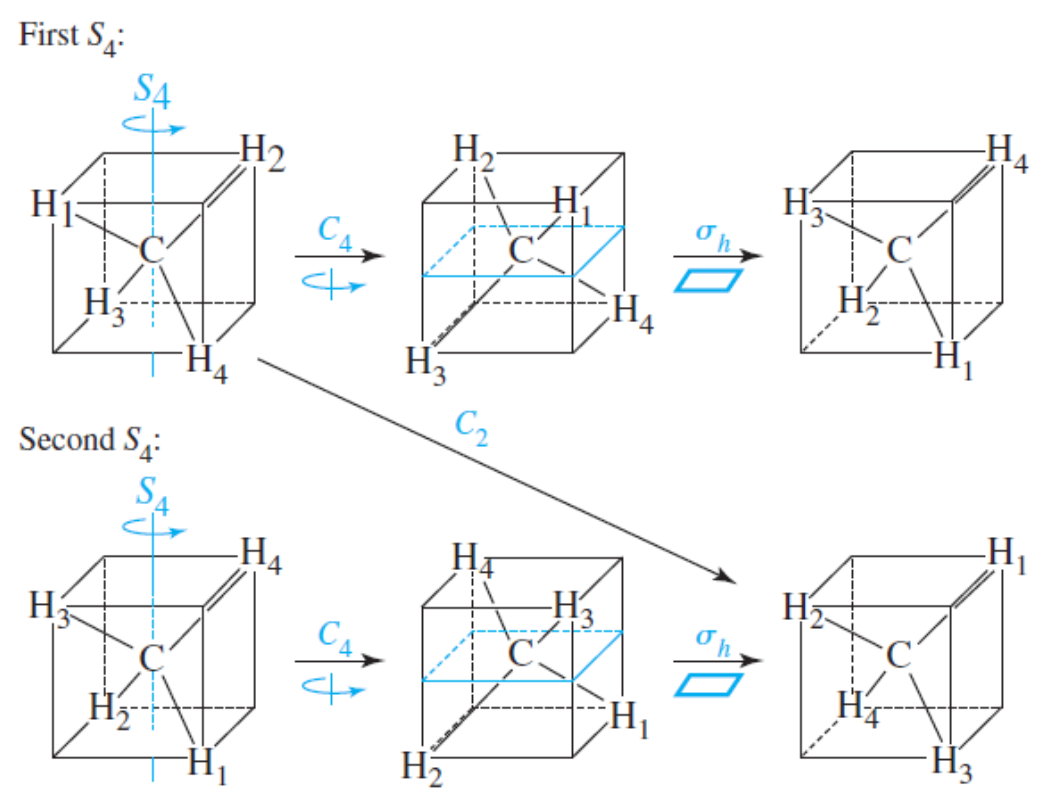
\includegraphics[width=0.4\linewidth]{../ExtFiles/methaneImproperRotation.png}
        \caption{Methane's $S_4$ symmetry.}
        \label{fig:methaneImproperRotation}
    \end{figure}
    \begin{itemize}
        \item Methane has $S_4$ symmetry.
        \item Note that $S_1\equiv\sigma_h$, $S_2\equiv i$, and sometimes $S_{2n}\equiv C_n$. In methane, for example, ${S_4}^2\equiv C_2$.
        \item Applied to a triangular prism, is a good example.
        \item If $n$ is even, we have $n$ unique operations. There should be $C_{n/2}$.
        \item If $n$ is odd, we have $2n$ unique operations. There should be $C_n$ and $\sigma_h$.
    \end{itemize}
    \item The absence of an $S_n$ axis is the defining symmetry property of \textbf{chiral} molecules.
    \begin{itemize}
        \item Formerly, we learned that chiral molecules should not have mirror planes and inversion centers.
        \item Rigorously, chiral molecules must not have any improper rotation axes.
    \end{itemize}
\end{itemize}



\section{Module 4: Symmetry Point Groups}
\begin{itemize}
    \item Identifying the point groups:
    \begin{enumerate}
        \item Determine if the symmetry is special (e.g., octahedral).
        \item Determine if there is a principal rotation axis.
        \item Determine if there are rotation axes perpendicular to the principal axis.
        \item Determine if there are mirror planes.
        \item Assign point groups.
    \end{enumerate}
    \item High symmetry and low symmetry groups are the most difficult to identify.
    \item High symmetry:
    \begin{itemize}
        \item Perfect tetrahedral ($T_d$), e.g., \ce{P4} and \ce{CH4}.
        \item Perfect octahedral ($O_h$), e.g., \ce{SF6}.
        \item Perfect icosahedral ($I_h$), e.g., \ce{C60} and \ce{B12H12^2-}.
    \end{itemize}
    \item Low symmetry:
    \begin{figure}[h!]
        \centering
        \begin{subfigure}[b]{0.24\linewidth}
            \centering
            \footnotesize
            \chemfig[cram dash width=0.5pt,cram dash sep=1.3pt,atom sep=7mm]{*8(<(<[:-120]F_3)=>(>:[:-30]F_2)=<(<[:60]F_1)=>(>:[:150]F_4)=)}
            \caption{$S_4$.}
            \label{fig:lowSymmetrya}
        \end{subfigure}
        \begin{subfigure}[b]{0.24\linewidth}
            \centering
            \footnotesize
            \chemfig{Cl-[1]C(<[:120]H)(>:[:60]F)-[7]Cl}
            \caption{$C_s$}
            \label{fig:lowSymmetryb}
        \end{subfigure}
        \begin{subfigure}[b]{0.24\linewidth}
            \centering
            \footnotesize
            \chemfig{H-[1]C(>:[3]Br)(<[:170]Cl)-C(<[7]Br)(>:[:-10]Cl)-[1]H}
            \caption{$C_i$}
            \label{fig:lowSymmetryc}
        \end{subfigure}
        \begin{subfigure}[b]{0.24\linewidth}
            \centering
            \footnotesize
            \chemfig{C(-[:-30]Br)(<[:-110]Cl)(>:[:-150]F)-[2]H}
            \caption{$C_1$}
            \label{fig:lowSymmetryd}
        \end{subfigure}
        \caption{Low symmetry point groups.}
        \label{fig:lowSymmetry}
    \end{figure}
    \begin{itemize}
        \item Only an improper axis: $S_n$.
        \item Only a mirror plane: $C_s$.
        \item Only an inversion center: $C_i$.
        \item No symmetry: $C_1$.
    \end{itemize}
    \item $C_n$ groups:
    \begin{itemize}
        \item Only a $C_n$ axis. Note that conformation is important.
    \end{itemize}
    \item $C_{nh}$ groups have a $C_n$ axis and a $\sigma_h$ reflection plane (such as \ce{B(OH)3}).
    \begin{itemize}
        \item \ce{H2O2} has $C_{2h}$ symmetry.
    \end{itemize}
    \item All symmetry elements are listed in the top row of the corresponding characters table (Appendix C in \textcite{bib:MiesslerFischerTarr}).
    \item $C_{nv}$ groups have a $C_n$ axis and a $\sigma_v$ reflection plane.
    \begin{itemize}
        \item \ce{NH3} has $C_{3v}$ symmetry.
        \item \ce{CO} has $C_{\infty v}$ symmetry since there are an infinite number of both $C_n$ axes and $\sigma_v$ mirror planes.
    \end{itemize}
    \item $D_{nh}$ groups: A $C_n$ axis, $n$ perpendicular $C_2$ axes, and a $\sigma_h$ reflection plane.
    \begin{itemize}
        \item \ce{BH3} has $D_{3h}$ symmetry.
        \item A square prism has $D_{4h}$ symmetry.
        \item \ce{CO2} has $D_{\infty h}$ symmetry.
    \end{itemize}
    \item $D_n$ groups: A $C_n$ axis, $n$ perpendicular $C_2$ axes, and no mirror planes.
    \begin{itemize}
        \item A 3-bladed propeller has $D_3$ symmetry.
    \end{itemize}
    \item $D_{nd}$ groups: A $C_n$ axis, $n$ perpendicular $C_2$ axes, and a $\sigma_d$.
    \begin{itemize}
        \item Ethane in the staggered conformation has $D_{3d}$ symmetry.
    \end{itemize}
    \item Local symmetry:
    \begin{itemize}
        \item Sometimes, rigorous math analysis needs to be adjusted to physical reality.
        \item If a cyclopentane ring is bonded through the center to \ce{Mn(CO)3}, this molecule has only $C_s$ symmetry.
        \item However, spectroscopically, there is fast rotation about the \ce{Mn-Cp} bond. This means that the \ce{Mn(CO)3} fragment exhibits pseudo-$C_{3v}$ symmetry while the \ce{C5H5} ligand exhibits pseudo-$C_{5v}$ symmetry.
        \item Often, the absolute symmetry of a molecule is very low, but the interactions are far away from the centers of interest, and do not perturb them significantly.
        \item If we have platinum as a central atom bonded to two chlorines and two \ce{P(Et)3} groups, this molecule technically has $C_1$ symmetry due to the orientations of atoms within \ce{R} groups (staggered), but IR spectroscopy is characteristic of highly symmetric species ($D_{2h}$).
    \end{itemize}
\end{itemize}



\section{Module 5: Group Theory 101}
\begin{itemize}
    \item \marginnote{1/15:}\textbf{Group}: A set of elements together with an operation that combines any two of its elements to form a third element satisfying four conditions called the group axioms.
    \item \textbf{Closure}: All binary products must be members of the group.
    \item \textbf{Associativity}: Associative law of multiplication must hold.
    \item \textbf{Identity}: A group must contain the identity operator.
    \item \textbf{Inverse}: Every operator must have an inverse.
    \item The integers with the addition operation form a group, for example.
    \item History:
    \begin{itemize}
        \item Early group theory was driven by the quest for solutions of polynomial equations of degree 5 and above.
        \item Early 1800s: \'{E}variste Galois realized that the algebraic solution to a polynomial equation is related to the structure of a group of permutations associated with the roots off the polynomial, the Galois group of the polynomial.
        \begin{itemize}
            \item Link to Galois video \href{https://www.youtube.com/watch?v=Ct2fyigNgPY}{here}.
        \end{itemize}
        \item 1920s: Group theory was applied to physics and chemistry.
        \item 1931: It is often hard or even impossible to obtain a solution of the Schr\"{o}dinger equation --- however, a large part of qualitative results can be obtained by group theory. Almost all the rules of spectroscopy follow from the symmetry of a problem.
    \end{itemize}
    \item We will use group theory for describing symmetry of molecules. We will use group theory to understand the bonding and spectroscopic features of molecules.
    \item For us, a group consists of a set of symmetry elements (and associated symmetry operations) that completely describes the symmetry of a molecule.
    \item \textbf{Order} (of a group): The total number of elements (i.e., symmetry operations) in the group. \emph{Also known as} $\bm{h}$.
    \item Rule 1: Closure.
    \begin{figure}[h!]
        \centering
        \begin{tikzpicture}
            \footnotesize
            \fill [orange!80!yellow,opacity=0.2] (-2,-1.2) rectangle (2,1.4) node[black,opacity=1,right]{$\sigma_v'$};
            \fill [orange!50!yellow,opacity=0.35] (0,-1.2,-2) -- (0,1.4,-2) -- (0,1.4,2) -- (0,-1.2,2) node[black,opacity=1,right]{$\sigma_v$};
            \draw [very thick,-stealth] (0,1.4,0) -- (0,3,0) node[above]{$z$};
            \draw [yshift=2cm,very thick,arrows={->[scale width=0.6,flex=2]}] (-120:0.3cm and 0.1cm) arc[start angle=240,end angle=-70,x radius=0.3cm,y radius=0.1cm] node[xshift=-7mm,yshift=1mm]{$C_2$};
    
            \draw [thick] (-1,-0.6) node[circle,ball color=gray]{} node[below=1mm]{1} -- (0,0) node[circle,ball color=red,inner sep=5pt]{} -- (1,-0.6) node[circle,ball color=gray]{} node[below=1mm]{2};
    
            \draw [very thick,-stealth] (0.25,0,0) -- (1,0,0) node[right]{$y$};
            \draw [very thick,-stealth] (0,0.25,0) -- (0,1,0) node[above]{$z$};
            \draw [very thick,-stealth] (0,0,0.25) -- (0,0,1.3) node[below left=-1mm]{$x$};
        \end{tikzpicture}
        \caption{Symmetry elements for \ce{H2O}.}
        \label{fig:symmetry-H2O}
    \end{figure}
    \begin{itemize}
        \item \ce{H2O} is of the $C_{2v}$ point group (refer to Figure \ref{fig:symmetry-H2O}).
        \begin{itemize}
            \item Symmetry operations: $E$, $C_2$, $\sigma_{v(xz)}$, and $\sigma'_{v(yz)}$.
            \item $\sigma_v\cdot C_2=\sigma_v'=C_2\cdot\sigma_v$.
            \item The above property (order \emph{does not} matter) shows that $C_{2v}$ is an \textbf{Abelian group}.
        \end{itemize}
        \item \ce{NH3} is of the $C_{2v}$ point group.
        \begin{itemize}
            \item Symmetry operations: $E$, ${C_3}^+$, ${C_3}^-$, $\sigma_v$, $\sigma_v'$, and $\sigma_v''$.
            \item $\sigma_v''\cdot C_3=\sigma_v$, but $C_3\cdot\sigma_v''={C_3}^-={C_3}^2$.
            \item The above property (order \emph{does} matter) shows that $C_{3v}$ is a \textbf{non-Abelian group}.
        \end{itemize}
    \end{itemize}
    \item Rule 2: Associativity.
    \begin{itemize}
        \item \ce{H2O} is of the $C_{2v}$ point group (refer to Figure \ref{fig:symmetry-H2O}).
        \begin{align*}
            \sigma_v'C_2\sigma_v(1,2) &= \sigma_v'C_2(2,1)&
                \sigma_v'(C_2\sigma_v)(1,2) &= \sigma_v'E(1,2)&
                    (\sigma_v'C_2)\sigma_v(1,2) &= \sigma_v\sigma_v(1,2)\\
            &= \sigma_v'(1,2)&
                &= \sigma_v'(1,2)&
                    &= \sigma_v(2,1)\\
            &= (1,2)&
                &= (1,2)&
                    &= (1,2)
        \end{align*}
    \end{itemize}
    \item Rule 3: Identity.
    \item Rule 4: Inverse.
    \begin{itemize}
        \item For a $C_{2v}$ point group:
        \begin{align*}
            E\cdot E &= E&
            C_2\cdot C_2 &= E&
            \sigma_v\cdot\sigma_v &= E&
            \sigma_v'\cdot\sigma_v' &= E
        \end{align*}
    \end{itemize}
    \item Group multiplication tables.
    \begin{table}[H]
        \centering
        \renewcommand{\arraystretch}{1.4}
        \footnotesize
        \begin{tabular}{l|llll}
            \normalsize$C_{2h}$ & $\bm{E}$   & $\bm{C_2}$ & $\bm{\sigma_h}$ & $\bm{i}$\\
            \hline
            $\bm{E}$            & $E$        & $C_2$      & $\sigma_h$      & $i$\\
            $\bm{C_2}$          & $C_2$      & $E$        & $i$             & $\sigma_h$\\
            $\bm{\sigma_h}$     & $\sigma_h$ & $i$        & $E$             & $C_2$\\
            $\bm{i}$            & $i$        & $\sigma_h$ & $C_2$           & $E$\\
        \end{tabular}
        \caption{Group multiplication table for the $C_{2h}$ point group.}
        \label{tab:groupMultiplication-C2h}
    \end{table}
    \begin{itemize}
        \item Table \ref{tab:groupMultiplication-C2h} corresponds to the $C_{2h}$ point group, which has $E$, $C_2$, $\sigma_h$, and $i$ operations.
        \item Note that the operation in the top row is the one that's applied first, while the one in the left column will be applied second.
    \end{itemize}
    \item \textbf{Subgroup}: Fractional parts of groups that are groups, too.
    \begin{table}[h!]
        \centering
        \renewcommand{\arraystretch}{1.4}
        \footnotesize
        \begin{tabular}{l|llllll}
            \normalsize$C_{3v}$ & $\bm{E}$ & $\bm{C_3}$ & $\bm{{C_3}^2}$ & $\bm{\sigma_v}$ & $\bm{\sigma_v'}$ & $\bm{\sigma_v''}$\\
            \hline
            $\bm{E}$            & $E$ & $C_3$ & ${C_3}^2$ & $\sigma_v$ & $\sigma_v'$ & $\sigma_v''$\\
            $\bm{C_3}$          & $C_3$ & ${C_3}^2$ & $E$ & $\sigma_v''$ & $\sigma_v$ & $\sigma_v'$\\
            $\bm{{C_3}^2}$      & ${C_3}^2$ & $E$ & $C_3$ & $\sigma_v'$ & $\sigma_v''$ & $\sigma_v$\\
            $\bm{\sigma_v}$     & $\sigma_v$ & $\sigma_v'$ & $\sigma_v''$ & $E$ & $C_3$ & ${C_3}^2$\\
            $\bm{\sigma_v'}$    & $\sigma_v''$ & $\sigma_v$ & $\sigma_v'$ & $C_3$ & ${C_3}^2$ & $E$\\
            $\bm{\sigma_v''}$   & $\sigma_v'$ & $\sigma_v''$ & $\sigma_v$ & ${C_3}^2$ & $E$ & $C_3$\\
        \end{tabular}
        \begin{tikzpicture}[remember picture,overlay]
            \draw [red,thick] (-6.75,1.73) rectangle (-4.9,0.75);
            \draw [blue,thick] (-6.78,1.76) rectangle (-3.9,0.3);
            \draw [red!50!blue,thick] (-6.81,1.79) rectangle (-2.9,-0.15);
        \end{tikzpicture}
        \caption{Group multiplication table for the $C_{3v}$ point group.}
        \label{tab:groupMultiplication-C3v}
    \end{table}
    \begin{itemize}
        \item If $h=6$ (as in the $C_{3v}$ group), subgroup order can be $h={\color{red!50!blue}3},{\color{blue}2},{\color{red}1}$. Why only these?
        \item The order ${\color{red}1}$ and ${\color{red!50!blue}3}$ charts are subgroups.
        \item The order ${\color{blue}2}$ chart is not a subgroup because ${C_3}^2$ is not an operation in the group (therefore, the "subgroup" is not closed).
    \end{itemize}
    \item We use subgroups because they can make complex problems simpler.
    \begin{itemize}
        \item For example, calculating the vibrational modes of \ce{CO2}.
        \item As another example, $D_{2h}$ is a subgroup of $D_{\infty h}$.
    \end{itemize}
\end{itemize}



\section{Module 6: Representations}
\begin{itemize}
    \item Items of the same point group have the same vibration modes.
    \item \textbf{Representation} (of a group): Any collection of quantities (or symbols) which obey the multiplication table of a group. \emph{Also known as} $\Gamma$.
    \item For our purposes, these quantities are the matrices that show how certain characteristic of a molecule behave under the symmetry operations of the group.
    \item Operations (on a point $(x,y,z)$ in Cartesian coordinates):
    \begin{itemize}
        \item $E(x,y,z)=(x,y,z)$.
        \item $\sigma_{xz}(x,y,z)=(x,-y,z)$.
        \item $i(x,y,z)=(-x,-y,-z)$.
        \item $C_n$: Convention is a counterclockwise rotation of the point by $\theta=\frac{2\pi}{n}$ radians.
        \item $S_n$: Convention is a clockwise rotation of the point $C_n$ followed by a $\sigma$ through a plane perpendicular to $C$.
    \end{itemize}
    \item Matrix forms of operations:
    \begin{itemize}
        \item Identity: $
            E =
            \begin{bmatrix}
                1 & 0 & 0\\
                0 & 1 & 0\\
                0 & 0 & 1\\
            \end{bmatrix}
        $.
        \item One example of a reflection (there are two more): $
            \sigma_{xy} =
            \begin{bmatrix}
                1 & 0 & 0\\
                0 & 1 & 0\\
                0 & 0 & -1\\
            \end{bmatrix}
        $.
        \item Inversion: $
            i =
            \begin{bmatrix}
                -1 & 0 & 0\\
                0 & -1 & 0\\
                0 & 0 & -1\\
            \end{bmatrix}
        $.
        \item Rotation: Counterclockwise is $
            C_n(\theta) =
            \begin{bmatrix}
                \cos\theta & -\sin\theta & 0\\
                \sin\theta & \cos\theta & 0\\
                0 & 0 & 1\\
            \end{bmatrix}
        $ and clockwise is $
            C_n(\theta) =
            \begin{bmatrix}
                \cos\theta & \sin\theta & 0\\
                -\sin\theta & \cos\theta & 0\\
                0 & 0 & 1\\
            \end{bmatrix}
        $.
        \begin{itemize}
            \item A derivation of this matrix can be found in the slides.
        \end{itemize}
        \item Improper rotation: $S_n(\theta)=\sigma_hC_n(\theta)$.
    \end{itemize}
    \item \textbf{Reducible representations} ($\Gamma$):
    \begin{itemize}
        \item A representation of a symmetry operation of a group.
        \item Can be expressed in terms of a representation of lower dimension.
        \item Can be broken down into a simpler form.
        \item Characters can be further diagonalized.
        \item Are composed of the direct sum of irreducible representations.
        \item Infinite possibilities.
    \end{itemize}
    \item \textbf{Irreducible representations} ($\Gamma_i$):
    \begin{itemize}
        \item A fundamental representation of a symmetry operation of a group.
        \item Cannot be expressed in terms of a representation of lower dimension.
        \item Cannot be broken down into a simpler form.
        \item Characters cannot be further diagonalized.
        \item Small finite number dictated by point group.
    \end{itemize}
    \item Good example of reducible/irreducible representations?
    \item A representation shows how certain characteristics of an object (a basis) behave under the symmetry operation of the group.
    \item \textbf{Conjugate elements}: Two elements $X$ and $Y$ for which there exists an element $Z$ in the group such that
    \begin{equation*}
        Z^{-1}\cdot X\cdot Z = Y
    \end{equation*}
    \begin{itemize}
        \item Every element is conjugated with itself (let $Z=E$).
        \item If $X$ is conjugated with $Y$, then $Y$ is conjugated with $X$.
        \item If $X$ is conjugated with $Y$ and $W$, then $Y$ and $W$ are also conjugate.
    \end{itemize}
    \item \textbf{Class}: A complete set of elements of a group that are conjugate to one another.
    \begin{itemize}
        \item Geometric meaning: operations in the same class can be converted into one another by changing the axis system through application of some symmetry operation of the group.
    \end{itemize}
    \item Find the conjugates to $C_3$ in the $C_{3v}$ point group (refer to Table \ref{tab:groupMultiplication-C3v} throughout the following discussion).
    \begin{itemize}
        \item Let $X=C_3$, let $Z$ iterate through the six symmetry elements ($E,C_3,{C_3}^2,\sigma_v,\sigma_v',\sigma_v''$), and let $Z^{-1}$ iterate through the corresponding inverses ($E,{C_3}^2,C_3,\sigma_v,\sigma_v',\sigma_v''$).
        \item Thus, we have
        \begin{gather*}
            E\cdot C_3\cdot E = C_3\\
            {C_3}^2\cdot C_3\cdot C_3 = C_3\\
            C_3\cdot C_3\cdot {C_3}^2 = C_3\\
            \sigma_v\cdot C_3\cdot\sigma_v = {C_3}^2\\
            \sigma_v'\cdot C_3\cdot\sigma_v' = {C_3}^2\\
            \sigma_v''\cdot C_3\cdot\sigma_v'' = {C_3}^2
        \end{gather*}
        \item It follows from the above that $C_3$ and $C_3$ are conjugates, and $C_3$ and ${C_3}^2$ are conjugates.
        \item Thus, $C_3$ and ${C_3}^2$ are in the same class.
        \item We can use a similar method to prove that $\sigma_v$, $\sigma_v'$, and $\sigma_v''$ are all in the same class within the $C_{3v}$ point group.
        \item Likewise $E$ is in a class by itself.
        \item Thus, for the $C_{3v}$ point group, $E$ forms a class of order 1, $C_3,{C_3}^2$ form a class of order 2, and $\sigma_v,\sigma_v',\sigma_v''$ form a class of order 3.
    \end{itemize}
    \item \textbf{Similarity transformation}: The transformation
    \begin{equation*}
        v^{-1}\cdot A\cdot v = A'
    \end{equation*}
    \begin{itemize}
        \item $A$ is a representation for some type of symmetry operation.
        \item $v$ is a similarity transform operator.
        \item $v^{-1}$ is the inverse of the similarity transform operator.
        \item $A'$ is the product.
        \item $A$ and $A'$ are conjugates, and we say that $A'$ is the similarity transform of $A$ by $v$.
    \end{itemize}
    \item \textbf{Block-diagonal} (matrix): A matrix with nonzero values only in square blocks along the diagonal from the top left to the bottom right.
    \begin{equation*}
        \begin{bmatrix}
            2 & 3 & 0 & 0 & 0\\
            1 & 2 & 0 & 0 & 0\\
            0 & 0 & 1 & 1 & 0\\
            0 & 0 & 1 & 1 & 0\\
            0 & 0 & 0 & 0 & 2\\
        \end{bmatrix}
    \end{equation*}
    \begin{itemize}
        \item The above matrix is an example of a block-diagonal matrix.
    \end{itemize}
    \item Irreducible representations are the ones where the matrices have the most block-diagonalized form that they can.
\end{itemize}



\section{Module 7: Characters and Character Tables}
\begin{itemize}
    \item \marginnote{1/19:}Nocera Lecture 3 notes (on Canvas) explain how reducible and irreducible transformations are related to each other through the similarity transformations.
    \item For \ce{H2O}, each atom has 3 Cartesian coordinates, so our transformation matrix\footnote{Some values in it are negative because of the cosine/sine definition of a rotation matrix for $\theta=\ang{180}$.} is 9-square.
    \begin{itemize}
        \item However, we can also apply a smaller matrix to the molecule as a whole and invoke symmetry to find the position of the individual atoms.
    \end{itemize}
    \item \textbf{Characters} (of a representation): The traces (i.e., sums of the diagonal matrix elements) of the representation matrices for each operation. \emph{Also known as} $\bm{\chi}$.
    \begin{itemize}
        \item The character is an invariant for each type of symmetry operation (e.g., regardless of the axis about which a $C_n$ operation is performed, the trace of the corresponding matrix will be the same).
    \end{itemize}
    \item Common characters:
    \begin{itemize}
        \item $C_n$ character: $\chi=2\cos\theta+1$.
        \item $\sigma_v,\sigma_d$ character: $\chi=1$.
        \item $S_2\equiv i$ character: $\chi=-3$.
        \item $S_n$ character: $\chi=2\cos\theta-1$.
        \item $\perp C_2$ axes character: $\chi=-1$.
    \end{itemize}
    \item \textbf{Character table}: The collection of characters for a given irreducible representation, under the operations of a group. \emph{Also known as} \textbf{$\bm{\chi}$ table}.
    \begin{figure}[h!]
        \centering
        \renewcommand{\arraystretch}{1.2}
        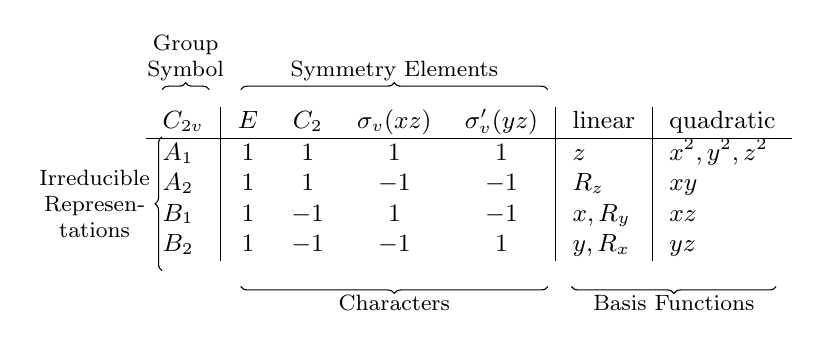
\begin{tikzpicture}
            \small
            \node {
                \begin{tabular}{l|cccc|l|l}
                    $C_{2v}$ & $E$ & $C_2$ & $\sigma_v(xz)$ & $\sigma_v'(yz)$ & linear  & quadratic\\
                    \hline
                    $A_1$    & $1$ & $1$   & $1$            & $1$             & $z$     & $x^2,y^2,z^2$\\
                    $A_2$    & $1$ & $1$   & $-1$           & $-1$            & $R_z$   & $xy$\\
                    $B_1$    & $1$ & $-1$  & $1$            & $-1$            & $x,R_y$ & $xz$\\
                    $B_2$    & $1$ & $-1$  & $-1$           & $1$             & $y,R_x$ & $yz$\\
                \end{tabular}
            };
    
            \footnotesize
            \draw [decorate,decoration=brace] (-3.9,1.2) -- node[above,text width=1cm,align=center]{Group Symbol} ++(0.6,0);
            \draw [decorate,decoration=brace] (-2.9,1.2) -- node[above]{Symmetry Elements} ++(3.9,0);
            \draw [decorate,decoration={brace,mirror}] (-3.9,0.6) -- node[left,text width=1.5cm,align=center]{Irreducible Representations} ++(0,-1.7);
            \draw [decorate,decoration={brace,mirror}] (-2.9,-1.3) -- node[below]{Characters} ++(3.9,0);
            \draw [decorate,decoration={brace,mirror}] (1.3,-1.3) -- node[below]{Basis Functions} ++(2.6,0);
        \end{tikzpicture}
        \caption{A character table.}
        \label{fig:characterTable}
    \end{figure}
    \begin{itemize}
        \item Character tables for all point groups are listed in Appendix C of \textcite{bib:MiesslerFischerTarr}.
    \end{itemize}
    \item \textbf{Mulliken symbols} are used to classify irreducible representations based on degeneracy and symmetry.
    \begin{itemize}
        \item A or B: singly degenerate (the maximum block size in the block-diagonalized irreducible transformation matrix is $1\times 1$).
        \item E: Doubly degenerate (the maximum block size in the block-diagonalized irreducible transformation matrix is $2\times 2$).
        \item T: Triply degenerate (the maximum block size in the block-diagonalized irreducible transformation matrix is $3\times 3$).
        \item A: symmetric ($+$) with respect to $C_n$.
        \item B: anti-symmetric ($-$) with respect to $C_n$.
        \item Subscript g: symmetric ($+$) with respect to $i$. \emph{Etymology} short for gerade (German for symmetric).
        \item Subscript u: anti-symmetric ($-$) with respect to $i$. \emph{Etymology} short for ungerade (German for unsymmetric).
        \begin{itemize}
            \item If the molecule has a center of inversion, we label irreducible representations with $g$ or $u$.
        \end{itemize}
        \item Subscript 1: symmetric ($+$) with respect to $\perp C_2$ or $\sigma_v$.
        \item Subscript 2: anti-symmetric ($-$) with respect to $\perp C_2$ or $\sigma_v$.
        \item Superscript $'$: symmetric ($+$) under $\sigma_h$ (if no $i$).
        \item Superscript $''$: anti-symmetric ($-$) under $\sigma_h$ (if no $i$).
    \end{itemize}
    \item Don't mistake the operation $E$ for the Mulliken symbol $E$!
    \item To assign Mulliken symbols, use the character table.
    \begin{itemize}
        \item Assigning the main letter:
        \begin{itemize}
            \item If $E\text{-character}=1$ and $C_n\text{-character}=1$: $A$.
            \item If $E\text{-character}=1$ and $C_n\text{-character}=-1$: $B$.
            \item If $E\text{-character}=2$: $E$.
            \item If $E\text{-character}=3$: $T$.
        \end{itemize}
        \item Assigning a subscript $g$ or $u$:
        \begin{itemize}
            \item If $i\text{-character}=1$: $g$.
            \item If $i\text{-character}=-1$: $u$.
            \item This subscript can be assigned to $A,B,E,T$ representations.
        \end{itemize}
        \item Assigning a superscript $'$ or $''$:
        \begin{itemize}
            \item If $\sigma_h\text{-character}=1$: $'$.
            \item If $\sigma_h\text{-character}=-1$: $''$.
            \item This subscript can be assigned to $A,B$ representations.
        \end{itemize}
        \item Assigning a subscript $1$ or $2$:
        \begin{itemize}
            \item If $\perp C_2\text{ or }\sigma_v\text{-character}=1$: $1$.
            \item If $\perp C_2\text{ or }\sigma_v\text{-character}=-1$: $2$.
            \item This subscript can be assigned to $A,B$ representations.
        \end{itemize}
    \end{itemize}
    \item $\sigma$, $\pi$, and $\delta$ bonds come from the Mulliken symbols!
    \begin{itemize}
        \item Infinity tables use Greek rather than Latin letters.
    \end{itemize}
    \begin{table}[h!]
        \centering
        \renewcommand{\arraystretch}{1.2}
        \small
        \begin{tabular}{l|ccc|l|l}
            $D_3$ & $E$ & $2C_3(z)$ & $3C_2'$ & \multicolumn{1}{c|}{linear} & \multicolumn{1}{c}{quadratic}\\
            \hline
            $A_1$ & $1$ & $1$ & $1$ & & $x^2+y^2,z^2$\\
            $A_2$ & $1$ & $1$ & $-1$ & $z,R_z$ & \\
            $E$ & $2$ & $-1$ & $0$ & $(x,y)(R_x,R_y)$ & $(x^2-y^2,xy)(xz,yz)$.
        \end{tabular}
        \caption{Character table for the $D_3$ point group.}
        \label{tab:characterTable-D3}
    \end{table}
    \item In character tables, we need to multiply each symmetry operation by the number of types there are (see Table \ref{tab:characterTable-D3}).
    \item Basis functions show us how different functions transform under different symmetry operations.
    \item In the $C_{2v}$ point group:
    \begin{itemize}
        \item The $p_x$ orbital has $B_1$ symmetry.
        \item $p_x$ transforms as $B_1$.
        \item $p_x$ has the same symmetry as $B_1$.
        \item $p_x$ forms a basis for the $B_1$ irreducible representation.
        \item $p_x$ is $B_1$ because (see Table \ref{tab:WaveFunctionsAngular-H} and Figure \ref{fig:characterTable}) it does not change under $E$, it inverts under $C_2$, it does not change under $\sigma_v(xz)$, and it inverts under $\sigma_v'(yz)$.
    \end{itemize}
    \item We can apply the same procedure to other more complex functions.
    \begin{itemize}
        \item For example, in the $C_{2v}$ point group, we know that (with respect to orbitals):
        \begin{itemize}
            \item $p_y$ is $B_2$.
            \item $p_z$ is $A_1$.
            \item $d_{z^2}$ is $A_1$.
            \item $d_{x^2-y^2}$ is $A_1$.
            \item $d_{yz}$ is $B_2$.
            \item $d_{xy}$ is $A_2$.
            \item $d_{xz}$ is $B_1$.
            \item We can even go into the cubic functions describing the $f$ orbitals and assign them Mulliken symbols.
        \end{itemize}
    \end{itemize}
    \item Essentially, the right hand side of a character table tells you how atomic orbitals will transform under certain symmetry operations.
    \item Properties of a character table:
    \begin{enumerate}
        \item The characters of all matrices belonging to the operations in the same class are identical in a given irreducible representation.
        \begin{itemize}
            \item As such, we form \textbf{classes} of operations.
            \item We most commonly form a \textbf{rotational class} and a \textbf{reflection class}.
        \end{itemize}
        \item The number of irreducible representations in a group is equal to the number of classes of that group.
        \item There is always a totally symmetric representation for any group.
        \begin{itemize}
            \item I.e., a representation where every character is $1$.
        \end{itemize}
        \item The sum of the squares of the \textbf{dimensionality} of all the irreducible representations is equal to the order of the group. Mathematically,
        \begin{equation*}
            h = \sum_i[\chi_i(E)]^2
        \end{equation*}
        \begin{itemize}
            \item For example, the dimensionalities of the $D_3$ point group (see Table \ref{tab:characterTable-D3}) are 1, 1, and 2, and the order is, indeed, $6=1^2+1^2+2^2$.
        \end{itemize}
        \item The sum of the squares of the characters multiplied by the number of operations in the class equals the order of the group. Mathematically,
        \begin{equation*}
            h = \sum_{R_c}g_c[\chi_i(R_c)]^2
        \end{equation*}
        \begin{itemize}
            \item For example, with respect to the $D_3$ point group (see Table \ref{tab:characterTable-D3}),
            \begin{align*}
                6 &= (1)(1)^2+(2)(1)^2+(3)(1)^2\\
                &= (1)(1)^2+(2)(1)^2+(3)(-1)^2\\
                &= (1)(2)^2+(2)(-1)^2+(3)(0)^2
            \end{align*}
        \end{itemize}
        \item The sum of the products of the corresponding characters of any two different irreducible representations of the same group is zero. Mathematically,
        \begin{equation*}
            \sum_{R_c}g_c\chi_i(R_c)\chi_f(R_c) = 0
        \end{equation*}
        \begin{itemize}
            \item Basically, this means that if we treat irreducible representations as vectors in $h$-space, they are orthogonal.
            \item For example, with respect to the $D_3$ point group (see Table \ref{tab:characterTable-D3}),
            \begin{align*}
                0 &= 1(1)(1)+2(1)(1)+3(1)(-1)\\
                &= 1(1)(2)+2(1)(-1)+3(1)(0)\\
                &= 1(1)(2)+2(1)(-1)+3(-1)(0)
            \end{align*}
        \end{itemize}
    \end{enumerate}
    \item \textbf{Dimensionality}: The character of the identity operation $E$. \emph{Also known as} \textbf{dimension}.
\end{itemize}



\section{Module 8: Using Character Tables}
\begin{itemize}
    \item A reducible representation of a group is any representation $\Gamma$ of the form
    \begin{equation*}
        \Gamma = \sum_ia_i\Gamma_i
    \end{equation*}
    where each $\Gamma_i$ is an irreducible representation of the group and $a_i$ is a real scalar.
    \begin{itemize}
        \item Basically, a reducible representation is any nontrivial linear combination of irreducible representations.
        \item For example, with respect to the $C_{2v}$ point group (see Figure \ref{fig:characterTable}), $\Gamma=(7,1,5,3)=4A_1+2B_1+B_2$ is a reducible representation.
    \end{itemize}
    \item We may "factor" reducible representations by inspection, or by the\dots
    \item Decomposition/reduction formula for a reducible representation:
    \begin{equation*}
        a_i = \frac{1}{h}\sum_QN\cdot\chi(R)_Q\cdot\chi_i(R)_Q
    \end{equation*}
    \begin{itemize}
        \item $a_i$ is the number of times the irreducible representation appears in $\Gamma_1$.
        \item $h$ is the order of the group.
        \item $N$ is the number of operations in class $Q$.
        \item $\chi(R)_Q$ is the character of the reducible representation.
        \item $\chi_i(R)_Q$ is the character of the irreducible representation.
        \item This formula cannot be applied to $D_{\infty h}$ and $C_{\infty v}$.
    \end{itemize}
    \item Let's look at decomposing $\Gamma=(7,1,5,3)$ into its component irreducible point groups using the above formula.
    \begin{align*}
        a_{A_1} &= \frac{1}{4}(1\cdot 7\cdot 1+1\cdot 1\cdot 1 +1\cdot 5\cdot 1 +1\cdot 3\cdot 1 ) = 4\\
        a_{A_2} &= \frac{1}{4}(1\cdot 7\cdot 1+1\cdot 1\cdot 1 +1\cdot 5\cdot -1+1\cdot 3\cdot -1) = 0\\
        a_{B_1} &= \frac{1}{4}(1\cdot 7\cdot 1+1\cdot 1\cdot -1+1\cdot 5\cdot 1 +1\cdot 3\cdot -1) = 2\\
        a_{B_2} &= \frac{1}{4}(1\cdot 7\cdot 1+1\cdot 1\cdot -1+1\cdot 5\cdot -1+1\cdot 3\cdot 1 ) = 1
    \end{align*}
    \item You can also find \href{http://symmetry.jacobs-university.de/}{websites} that will apply the formula for you.
    \item Basis $\to$ reducible representation $\to$ irreducible representations workflow:
    \begin{enumerate}
        \item Assign a point group.
        \item Choose a basis function (bond, vibration, orbital, angle, etc.).
        \item Apply operations.
        \begin{itemize}
            \item The following shortcuts allow us to skip matrix math in certain situations.
            \begin{itemize}
                \item If the basis stays the same: $+1$.
                \item If the basis is reversed: $-1$.
                \item If it is a more complicated change: $0$.
            \end{itemize}
        \end{itemize}
        \item Generate a reducible representation.
        \item Reduce to irreducible representation.
    \end{enumerate}
    \item We now look at an example of applying the above method to \ce{H2O}.
    \begin{itemize}
        \item \ce{H2O} is of the $C_{2v}$ point group.
        \item The $9\times 9$ identity matrix represents the identity operation on the 3 atoms in \ce{H2O}, each described by 3 Cartesian coordinates. Thus, $\chi(E)=9$.
        \item The following matrix represents the $C_2$ symmetry operation. Thus, $\chi(C_2)=-1$.
        \begin{center}
            \begin{tikzpicture}
                \node {$
                    \begin{bmatrix}
                        x'\\
                        y'\\
                        z'\\
                        x'\\
                        y'\\
                        z'\\
                        x'\\
                        y'\\
                        z'\\
                    \end{bmatrix}
                    =
                    \begin{bmatrix}
                        -1 & 0 & 0 & 0 & 0 & 0 & 0 & 0 & 0\\
                        0 & -1 & 0 & 0 & 0 & 0 & 0 & 0 & 0\\
                        0 & 0 & 1 & 0 & 0 & 0 & 0 & 0 & 0\\
                        0 & 0 & 0 & 0 & 0 & 0 & -1 & 0 & 0\\
                        0 & 0 & 0 & 0 & 0 & 0 & 0 & -1 & 0\\
                        0 & 0 & 0 & 0 & 0 & 0 & 0 & 0 & 1\\
                        0 & 0 & 0 & -1 & 0 & 0 & 0 & 0 & 0\\
                        0 & 0 & 0 & 0 & -1 & 0 & 0 & 0 & 0\\
                        0 & 0 & 0 & 0 & 0 & 1 & 0 & 0 & 0\\
                    \end{bmatrix}
                    \begin{bmatrix}
                        x\\
                        y\\
                        z\\
                        x\\
                        y\\
                        z\\
                        x\\
                        y\\
                        z\\
                    \end{bmatrix}
                $};
        
                \draw [decorate,decoration=brace] (-4.3,-1.9) -- node[left]{\ce{H_b}} ++(0,1.2);
                \draw [decorate,decoration=brace] (-4.3,-0.6) -- node[left]{\ce{H_a}} ++(0,1.2);
                \draw [decorate,decoration=brace] (-4.3,0.7) -- node[left]{\ce{O}} ++(0,1.2);
        
                \draw [decorate,decoration={brace,mirror}] (4.3,-1.9) -- node[right]{\ce{H_b}} ++(0,1.2);
                \draw [decorate,decoration={brace,mirror}] (4.3,-0.6) -- node[right]{\ce{H_a}} ++(0,1.2);
                \draw [decorate,decoration={brace,mirror}] (4.3,0.7) -- node[right]{\ce{O}} ++(0,1.2);
            \end{tikzpicture}
        \end{center}
        \begin{itemize}
            \item Note that atoms moved during the transformation do not contribute to the character of the transformation matrix.
        \end{itemize}
        \item Since under $\sigma_v(xz)$ only \ce{O} is unshifted, we need only consider its part of the transformation matrix (as follows) when looking for the character. Thus, $\chi(\sigma_v(xz))=1$\footnote{Note also that $a_{11}=1$ since the $x$-vector (a basis) is unchanged under $\sigma_v(xz)$, $a_{22}=-1$ since the $y$-vector is reversed under $\sigma_v(xz)$, and $a_{33}=1$ since the $z$ vector is unchanged under $\sigma_v(xz)$.}.
        \begin{equation*}
            \begin{bmatrix}
                x'\\
                y'\\
                z'\\
            \end{bmatrix}
            =
            \begin{bmatrix}
                1 & 0 & 0\\
                0 & -1 & 0\\
                0 & 0 & 1\\
            \end{bmatrix}
            \begin{bmatrix}
                x\\
                y\\
                z\\
            \end{bmatrix}
        \end{equation*}
        \item Since under $\sigma_v(yz)$ no atom is shifted, we need to consider each (identical) part of the transformation matrix (as follows) when looking for the character. Thus, $\chi(\sigma_v(yz))=3$.
        \begin{equation*}
            \begin{bmatrix}
                x'\\
                y'\\
                z'\\
            \end{bmatrix}
            =
            \begin{bmatrix}
                -1 & 0 & 0\\
                0 & 1 & 0\\
                0 & 0 & 1\\
            \end{bmatrix}
            \begin{bmatrix}
                x\\
                y\\
                z\\
            \end{bmatrix}
        \end{equation*}
        \item Thus, the characters of our final reducible representation is $\Gamma_{3N}=(9,-1,1,3)$.
        \begin{itemize}
            \item This representation represents fully unrestricted motion of all 3 ambiguities of freedom.
        \end{itemize}
    \end{itemize}
    \item Another example: \ce{XeOF4}.
    \begin{figure}[h!]
        \centering
        \chemfig{Xe(>:[:30]F_c)(=[2]O)(>:[:150]F_d)(<[:-150]F_a)<[:-30]F_b}
        \caption{\ce{XeOF4}.}
        \label{fig:XeOF4}
    \end{figure}
    \begin{itemize}
        \item Point group: $C_{4v}$.
        \item Basis function: \ce{F} atoms.
        \item Let's see what happens to the fluorine atoms under the $C_{4v}$ operations (remember that if a basis element (a fluroine atom) stays the same, it contributes $+1$ to the character of an operation, and if it moves, it contributes $0$ to the character).
        \begin{table}[H]
            \centering
            \begin{tabular}{lll}
                $E$ & all unchanged & $4$\\
                $C_4$ & all move & $0$\\
                $C_2$ & all move & $0$\\
                $2\sigma_v$ & 2 move, 2 unchanged & $2$\\
                $2\sigma_d$ & all move & $0$\\
            \end{tabular}
            \caption{Changes in the fluorine atoms of \ce{XeOF4} under the $C_{4v}$ symmetry operations.}
            \label{tab:XeOF4-operationResults}
        \end{table}
        \item Thus, $\Gamma=(4,0,0,2,0)$.
        \item With the $C_{4v}$ character table and the decomposition formula, we can discover that $\Gamma=A_1+B_1+E$.
    \end{itemize}
\end{itemize}



\section{TA Review Session 1}
\begin{itemize}
    \item \marginnote{1/22:}We also don't need to show the equatorial electron pair in the shape picture.
    \item For \ce{SeCl4}, we need to show that the axial bonds are longer and are not straight up and down.
    \item For \ce{I3-}, it's trigonal bipyrimidal EPA and linear molecular geometry --- there's an extra electron pair around the central iodine atom. This makes it $D_{\infty h}$ point group.
    \item For \ce{SeOCl4}, we should also make the axials longer and bent away from the oxygen atom.
    \begin{itemize}
        \item This molecule is $sp^3d$ hybridized, not $sp^2d^2$, as it would be if the oxygen were axial.
    \end{itemize}
    \item For \ce{IO(OH)5}, we should show the equatorial \ce{OH}'s pushed away from the oxygen atom. The oxygen bond should also be a bit shorter.
    \item In the exam, they will specify whether we need to consider the hydrogens or not when calculating symmetry.
    \item For \ce{ClOF4-}, one or the other of the lone pair/oxygen will push the equatorial fluorines a bit. You don't have to know witch, just show bent.
    \item For \ce{XeO2F2}, show the lone pair pushing the axial fluorines away.
    \item For \ce{IF3^2-}, show that this is a \emph{distorted} T.
    \item A tennis ball belongs to the $D_{2d}$ point group since you have perpendicular $C_2$ axes punching through the seam and mirror planes at $\ang{45}$ angles to the $C_2$ axes (i.e., dihedral).
    \item \ce{FeF6^3-} also loses 4 $C_2$ axes.
    \item There are three possible isomers of \ce{IF3O2} (see Figure \ref{fig:VSEPR-BrF3}), but the one with equatorial oxygens is the most stable.
    \begin{itemize}
        \item The structure analogous to Figure \ref{fig:VSEPR-BrF3a} has $C_{2v}$ symmetry.
        \item The structure analogous to Figure \ref{fig:VSEPR-BrF3b} has $D_{3h}$ symmetry.
        \item The structure analogous to Figure \ref{fig:VSEPR-BrF3c} has $C_s$ symmetry.
    \end{itemize}
    \item Determine the point group of \ce{NO3^2-}, \ce{HFC=C=CHF}, \ce{H2C=CF2}, and \ce{C2H6} (consider three possible conformers).
    \begin{itemize}
        \item \ce{NO3^2-} is of the $D_{3h}$ point group.
        \item \ce{HFC=C=CHF} is of the $C_2$ point group.
        \item \ce{H2C=CF2} is of the $C_{2v}$ point group.
        \item \ce{C2H6} eclipsed has $D_{3h}$ symmetry, staggered has $D_{3d}$ symmetry, and others have $D_3$ symmetry.
    \end{itemize}
\end{itemize}



\section{Module 9: Molecular Vibrations}
\begin{itemize}
    \item \marginnote{1/25:}If you have a nonlinear triatomic molecule (like \ce{H2O}), we have $3\text{ atoms}\times 3\text{ DOF}=9\text{ DOF}$.
    \begin{itemize}
        \item This accounts for any possible perturbations of our molecules.
    \end{itemize}
    \item We can break this down into three types of motion:
    \begin{itemize}
        \item Translational motion along the $x$-, $y$-, and $z$-axes (3 DOFs).
        \item Rotational motion about the $x$-, $y$-, and $z$-axes (3 more DOFs).
        \item The remaining degrees of freedom are vibrational.
    \end{itemize}
    \item Every \emph{nonlinear} molecule has 3 translational and 3 rotational DOFs.
    \begin{itemize}
        \item The number of vibrations is $3N-6$, where $N$ is the number of atoms.
    \end{itemize}
    \item Every \emph{linear} molecule has 3 translational and 2 rotational DOFs.
    \begin{itemize}
        \item The number of vibrations is $3N-5$, where $N$ is the number of atoms.
    \end{itemize}
    \item \textbf{Vibrational mode}: A perturbation of molecular structure that keeps the center of mass of the molecule in one place.
    \item For \ce{H2O}, there are three vibrational modes: antisymmetric stretch (one \ce{H} moves away from the \ce{O} as the other moves in, and then the process reverses), symmetric stretch (both \ce{H}'s move away from the \ce{O} and then move back in), and scissoring bend (the bond angle changes).
    \item For molecules in general, there are these three and an additional three: wagging (in \ce{H2O}, the \ce{H}'s rotate out of the plane of the molecule and then back), twisting (in \ce{H2O}, both \ce{H}'s rotate out of the plane of the molecule, but one in one direction and one in the other), and rocking (in \ce{H2O}, both \ce{H}'s rotate about the \ce{O} within the plane of the molecule preserving the bond angle, and then go back).
    \item What vibrational modes a molecule can and cannot have is governed by its point group and group theory.
    \item Each normal mode of vibration forms a basis for an irreducible representation of the point group of the molecule.
    \item Workflow to identify the vibrational properties of a molecule:
    \begin{enumerate}
        \item Find number/symmetry of vibrational modes.
        \item Assign the symmetry of known vibrations.
        \item What does the vibration look like?
        \item Find if a vibrational mode is IR or Raman Active.
    \end{enumerate}
    \item To find vibrational modes, follow the 5-step Basis $\to$ reducible representation $\to$ irreducible representation workflow and then subtract translational and rotational motion.
    \begin{itemize}
        \item For example, with \ce{H2O}, as before, we have $C_{2v}$ point group, $3N$ basis, $\Gamma_{3N}=(9,-1,1,3)$, and $\Gamma_{3N}=3A_1+A_2+2B_1+3B_2$.
        \item We now need to use the basis functions in the $C_{2v}$ character table to determine the translational and rotational degrees of freedom. From Figure \ref{fig:characterTable}, the $x,y,z$-translational modes come from the $B_1$, $B_2$, and $A_1$ $\Gamma_i$'s, respectively. Thus, the total translational mode, sufficient to describe all possible translations in 3 DOFs, is $\text{trans}=A_1+B_1+B_2$. Similarly, we can determine that the total rotational mode is $\text{rot}=A_2+B_1+B_2$.
        \item Thus, we can determine that the total vibrational mode is $\Gamma_{3N}-\text{trans}-\text{rot}=2A_1+B_2$.
        \item When \ce{H2O} scissors or symmetrically stretches, it maintains its $C_{2v}$ symmetry. Thus, both of these vibrations are represented by the totally symmetric irreducible representation $A_1$ (hence the $2A_1$ component).
        \item As to asymmetric stretch, there exist points in time where \ce{H2O} lowers its symmetry from $C_{2v}$ to $C_s$, losing its $C_2$ and $\sigma_v(xz)$ symmetry elements but maintaining $E$ and $\sigma_v(yz)$. This shift is encapsulated by the $B_2$ irreducible representation.
        \item We can see all of these modes in \ce{H2O}'s infrared absorption spectrum.
        \begin{itemize}
            \item Note that this spectrum does not tell us the energy of vibrations (we can model this with quantum mechanics), or if it is IR or Raman active (which modes will appear in the respective spectrum).
        \end{itemize}
    \end{itemize}
    \item Determine the number and symmetry types for the translations, vibrations, and rotations of \ce{PF5}.
    \begin{itemize}
        \item Point group: $D_{3h}$.
        \begin{table}[h!]
            \centering
            \small
            \renewcommand{\arraystretch}{1.2}
            \begin{tabular}{l|cccccc|l|l}
                $D_{3h}$ & $E$ & $2C_3$ & $3C_2$ & $\sigma_h$ & $2S_c$ & $3\sigma_v$ & linear & quadratic\\
                \hline
                $A_1'$ & 1 & 1 & 1 & 1 & 1 & 1 & & $x^2+y^2,z^2$\\
                $A_2'$ & 1 & 1 & $-1$ & 1 & 1 & $-1$ & $R_z$ & \\
                $E'$ & 2 & $-1$ & 0 & 2 & $-1$ & 0 & $(x,y)$ & $(x^2-y^2,xy)$\\
                $A_1''$ & 1 & 1 & 1 & $-1$ & $-1$ & $-1$ & & \\
                $A_2''$ & 1 & 1 & $-1$ & $-1$ & $-1$ & 1 & $z$ & \\
                $E''$ & 2 & $-1$ & 0 & $-2$ & 1 & 0 & $(R_x,R_y)$ & $(xz,yz)$\\
            \end{tabular}
            \caption{Character table for the $D_{3h}$ point group.}
            \label{tab:characterTable-D3h}
        \end{table}
        \item We could write out all 18 $x,y,z$-vectors, or we can use a shortcut: To construct $\Gamma_{3N}$, we can, for each symmetry element, multiply the number of atoms atoms unmoved under the operation by the corresponding character the representation that accounts for $x,y,z$-movements.
        \begin{equation*}
            \Gamma_{3N} = (\Gamma_{x,y,z})\cdot(\text{\# unmoved atoms})
        \end{equation*}
        Applying this shortcut, we have $\Gamma_{x,y,z}=E'+A_2''=(3,0,-1,1,-2,1)$. We also have $\text{\# unmoved atoms}=(6,3,2,4,1,4)$. Thus, $\Gamma_{3N}=(18,0,-2,4,-2,4)$.
        \item We can now reduce it into $\Gamma_{3N}=2A_1'+A_2'+4E'+3A_2''+2E''$.
        \begin{itemize}
            \item Note that we still have our 18 degrees of freedom because each $E$ is double degenerate, meaning that $4E'$ counts for 8 degrees of freedom and $2E''$ counts for 4 degrees of freedom.
        \end{itemize}
        \item This combined with the fact that $\Gamma_\text{trans}=\Gamma_{x,y,z}=E'+A_2''$ and $\Gamma_\text{rot}=A_2'+E''$ implies that $\Gamma_\text{vibs}=2A_1'+3E'+2A_2''+E''$.
        \begin{itemize}
            \item For a similar reason to the note above, we can count $12=3N-6$ degrees of freedom (vibrational modes) in $\Gamma_\text{vibs}$.
        \end{itemize}
        \item Although degenerate modes count for multiple DOFs, the multiple modes they count for are of the same type.
        \begin{itemize}
            \item In an ideal world, those modes corresponding to $E$ would be twice as intense as the others.
            \item From the definition of $\Gamma_\text{vibs}$ and the above discussion, we know that \ce{PF5} has $2+3+2+1=8$ distinct vibrational modes.
        \end{itemize}
    \end{itemize}
    \item There are (broadly) two types of vibrations: \textbf{stretches} ($\nu$) and \textbf{bends} ($\delta$).
    \begin{itemize}
        \item These two types appear in different energies in IR and Raman spectra.
    \end{itemize}
    \item To differentiate between stretching and bending modes: Look at how the stretching modes transform. Each stretch happens along a single vector from central atom to ligand. Thus, if we let these vectors be our basis and look at how many vectors stay the same ($+1$) or change ($-1$) under each operation, we will have a reducible representation that can be decomposed. Its components will be the stretching modes and $\Gamma_\text{vibs}-\Gamma_\nu$ will equal $\Gamma_\delta$.
    \begin{itemize}
        \item Applied to \ce{PF5}, we have $\Gamma_\nu=(5,2,1,3,0,3)=2A_1'+E'+A_2''$.
        \item Thus, both $A_1'$ representations, one $E'$ representation, and one $A_2''$ representation correspond to stretching modes. Consequently, the other two $E'$ representations, the other $A_2''$ representation, and the $E''$ representation correspond to bending modes.
    \end{itemize}
\end{itemize}



\section{Module 10: IR and Raman Active Vibrations}
\begin{itemize}
    \item Today, we will learn what we need to know for PSet 2. Tomorrow, we will introduce a more rigorous, quantum mechanical foundation.
    \item Molecular vibrations can be experimentally observed by \textbf{infrared spectroscopy} or \textbf{Raman spectroscopy}.
    \item \textbf{Infrared spectroscopy}: A method of measuring the change in dipole moment during a vibration\footnote{Refer to \textcite{bib:APChemNotes}, specifically the discussion of spectroscopy in Chapter 13.}. \emph{Also known as} \textbf{IR spectroscopy}.
    \item \textbf{Raman spectroscopy}: A method of measuring the change in the polarizability during a vibration. We impinge upon a sample of a substance with an incident light (a powerful laser). Most of the light that scatters will be a \textbf{Raleigh scatter}, but some will be a \textbf{Raman scatter} (a new wavelength).
    \item \textbf{Raleigh scatter}: The same wavelength is emitted as was impinged by the incident light because the laser was elastically scattered. The electrons fell the same number of energy levels that they rose after absorbing the light.
    \item \textbf{Raman scatter}: A new wavelength is emitted, different than the one impinged by the incident light. The electrons fell fewer (\textbf{Stokes Raman scattering}) or more (\textbf{Anti-Stokes Raman scattering}) energy levels than they rose after absorbing the light.
    \item \textbf{IR active} (vibration): A vibration that transforms with the same symmetry as the $\vec{x}$, $\vec{y}$, and $\vec{z}$ vectors (see the $\chi$ tables).
    \item \textbf{Raman active} (vibration): A vibration having the same symmetry as the quadratic $x,y,z$ terms, i.e., $x^2,z^2,yz$, etc.
    \item For molecules possessing inversion centers, IR and Raman activity will be mutually exclusive.
    \item Activity data comes from character tables.
    \begin{itemize}
        \item All vibration representations that have a linear term are IR active, while those that have a quadratic term are Raman active.
    \end{itemize}
    \item Continuing with the \ce{PF5} example\dots
    \begin{itemize}
        \item Table \ref{tab:characterTable-D3h} tells us that $E'$ and $A_2''$ vibrations are IR active, and $A_1'$, $E'$, and $E''$ are Raman active.
        \item Thus, since $\Gamma_\text{vibs}=2A_1'+3E'+2A_2''+E''$, there are $3+2=5$ IR active bonds (corresponding to $3\cdot 2+2=8$ vibrations) and $2+3+1=6$ Raman active bonds (corresponding to $2+3\cdot 2+1\cdot 2=10$ vibrations).
    \end{itemize}
\end{itemize}



\section{Chapter 4: Symmetry and Group Theory}
\emph{From \textcite{bib:MiesslerFischerTarr}.}
\begin{itemize}
    \item \marginnote{1/18:}\textbf{Coincident} (axes): Two identical axes.
    \begin{itemize}
        \item For example, the $C_3$ rotation axis of \ce{CHCl3} is \textbf{coincident} with the \ce{C-H} bond axis.
    \end{itemize}
    \item Snowflakes, which are often planar and have hexagonal symmetry, have a twofold ($C_2$), threefold ($C_3$), and sixfold ($C_6$) axis through their center and perpendicular to their plane.
    \begin{itemize}
        \item Rotations ${C_3}^2$ and ${C_6}^5$ are also symmetry operations.
    \end{itemize}
    \begin{figure}[h!]\marginnote{1/19:}
        \centering
        \begin{subfigure}[b]{0.3\linewidth}
            \centering
            \begin{tikzpicture}[decoration=Koch snowflake]
                \footnotesize
                \draw [gry,thick] (30:{2/3^0.5}) ++(90:1.3) -- ++(90:0.9);
                \draw [gry,thick] (30:{2/3^0.5}) ++(150:1.3) -- ++(150:0.3);
                \draw [gry,thick] (30:{2/3^0.5}) ++(210:1.3) -- ++(210:0.6);
                \draw [gry,thick] (30:{2/3^0.5}) ++(270:1.3) -- ++(270:0.9);
    
                \draw [gry,thick,-stealth] (30:{2/3^0.5}) ++(90:1.45) arc (90:150:1.45) node[black,below,xshift=-1mm]{$C_6$};
                \draw [gry,thick,-stealth] (30:{2/3^0.5}) ++(90:1.75) arc (90:210:1.75) node[black,below,xshift=1mm]{$C_3$};
                \draw [gry,thick,-stealth] (30:{2/3^0.5}) ++(90:2.05) arc (90:270:2.05) node[black,right]{$C_2$};
    
                \filldraw [draw=grx,thick,fill=grz] decorate{decorate{(0,0) -- ++(60:2) -- ++(-60:2) -- cycle}};
            \end{tikzpicture}
            \caption{About the principal axis.}
            \label{fig:snowflakeRotationa}
        \end{subfigure}
        \begin{subfigure}[b]{0.3\linewidth}
            \centering
            \begin{tikzpicture}[decoration=Koch snowflake]
                \footnotesize
                \path (30:{2/3^0.5}) ++(90:2.2) -- ++(90:-4.4);
    
                \draw [gry,thick] (30:{2/3^0.5}) ++(90:1.7) node[black,above]{${C_2}'$} -- ++(90:-3.4);
                \draw [gry,thick,-stealth] (30:{2/3^0.5}) ++(90:1.6) ++(110:3.5mm and 0.7mm) arc (110:330:3.5mm and 0.7mm);
                \draw [gry,thick,densely dashed] (30:{2/3^0.5}) ++(0:1.7) node[black,right]{${C_2}''$} -- ++(0:-3.4);
                \draw [gry,thick,-stealth] (30:{2/3^0.5}) ++(0:1.6) ++(20:0.7mm and 3.5mm) arc (20:240:0.7mm and 3.5mm);
    
                \filldraw [draw=grx,thick,fill=grz] decorate{decorate{(0,0) -- ++(60:2) -- ++(-60:2) -- cycle}};
            \end{tikzpicture}
            \caption{About perpendicular axes.}
            \label{fig:snowflakeRotationb}
        \end{subfigure}
        \caption{Rotations of a snowflake design.}
        \label{fig:snowflakeRotation}
    \end{figure}
    \item \marginnote{1/18:}"When necessary, the $C_2$ axes perpendicular to the principal axis are designated with primes; a single prime (${C_2}'$) indicates that the axis passes through several atoms of the molecule, whereas a double prime (${C_2}''$) indicates that it passes between the outer atoms" \parencite[77]{bib:MiesslerFischerTarr}.
    \item \marginnote{1/19:}Even though $S_2\equiv i$ and $S_1\equiv\sigma$, the $i$ and $\sigma$ notations are preferred because of the group theory requirement of maximizing the number of unique classes of symmetry operations associated with a molecule.
    \item \textbf{Point group}: A set of symmetry operations that describes a molecule's overall symmetry.
    \item Alternative steps for assigning point groups:
    \begin{enumerate}
        \item Determine whether the molecule exhibits very low symmetry ($C_1$, $C_s$, $C_i$) or high symmetry ($T_d$, $O_h$, $C_{\infty v}$, $D_{\infty h}$, $I_h$).
        \item If not, find the highest order $C_n$ axis for the molecule.
        \item Does the molecule have any $C_2$ axes perpendicular to the principal $C_n$ axis? If it does, there will be $n$ of such $C_2$ axes, and the molecule is in the $D$ set of groups. If not, it is in the $C$ or $S$ set.
        \item Does the molecule have a mirror plane ($\sigma_h$) perpendicular to the principal $C_n$ axis? If so, it is classified as $C_{nh}$ or $D_{nh}$. If not, continue with Step 5.
        \item Does the molecule have any mirror planes that contain the principal $C_n$ axis ($\sigma_v$ or $\sigma_d$)? If so, it is classified as $C_{nv}$ or $D_{nd}$. If not, but it is in the $D$ set, it is classified as $D_n$. If the molecule is in the $C$ or $S$ set, continue with Step 6.
        \item Is there an $S_{2n}$ axis collinear with the principal $C_n$ axis? If so, it is classified as $S_{2n}$. If not, the molecule is classified as $C_n$.
    \end{enumerate}
    \item Groups of high symmetry:
    \begin{itemize}
        \item $C_{\infty v}$ (linear): These molecules are linear, with an infinite number of rotations and an infinite number of reflection planes containing the rotation axis. They do not have a center of inversion.
        \item $D_{\infty h}$ (linear): These molecules are linear, with an infinite number of rotations and an infinite number of reflection planes containing the rotation axis. They also have perpendicular $C_2$ axes, a perpendicular reflection plane, and an inversion center.
        \item $T_d$ (tetrahedral): Most (but not all) molecules in this point group have the familiar tetrahedral geometry. They have four $C_3$ axes, three $C_2$ axes, three $S_4$ axes, and six $\sigma_d$ planes. They have no $C_4$ axes.
        \begin{itemize}
            \item Look for $C_3$ and $C_2$ axes.
        \end{itemize}
        \item $O_h$ (octahedral): These molecules include those of octahedral structure, although some other geometrical forms, such as the cube, share the same set of symmetry operations. Among their 48 symmetry operations are four $C_3$ rotations, three $C_4$ rotations, and an inversion.
        \begin{itemize}
            \item Look for $C_4$, $C_3$, and $C_2$ axes.
        \end{itemize}
        \item $I_h$ (icosahedral): Icosahedral structures are best recognized by their six $C_5$ axes, as well as many other symmetry operations --- 120 in all.
        \begin{itemize}
            \item Look for $C_5$, $C_3$, and $C_2$ axes.
        \end{itemize}
        \item $T_h$: Adds $i$ to $T_d$. Example: \ce{W[N(CH3)2]6}.
    \end{itemize}
    \item \marginnote{1/24:}When we have a block-diagonalized reducible representation, the irreducible representations can be obtained from the individual blocks.
    \begin{itemize}
        \item This is because we will find that an analogous set of blocks satisfies the multiplication table for the group.
    \end{itemize}
    \item For the $C_{2v}$ point group, we have the following reducible representation that can be applied to each coordinate.
    \begin{align*}
        E &:
        \begin{bmatrix}
            1 & 0 & 0\\
            0 & 1 & 0\\
            0 & 0 & 1\\
        \end{bmatrix}&
        C_2 &:
        \begin{bmatrix}
            -1 & 0 & 0\\
            0 & -1 & 0\\
            0 & 0 & 1\\
        \end{bmatrix}&
        \sigma_v(xz) &:
        \begin{bmatrix}
            1 & 0 & \\
            0 & -1 & 0\\
            0 & 0 & 1\\
        \end{bmatrix}&
        \sigma_v(yz) &:
        \begin{bmatrix}
            -1 & 0 & 0\\
            0 & 1 & 0\\
            0 & 0 & 1\\
        \end{bmatrix}
    \end{align*}
    \begin{itemize}
        \item The above matrices are block diagonalized. Thus, the sets of $a_{11}$, $a_{22}$ and $a_{33}$ form three irreducible representations (and we can confirm that these obey the $C_{2v}$ group multiplication table).
        \begin{align*}
            E &:
            \begin{bmatrix}
                1\\
            \end{bmatrix}&
                C_2 &:
                \begin{bmatrix}
                    -1\\
                \end{bmatrix}&
                    \sigma_v(xz) &:
                    \begin{bmatrix}
                        1\\
                    \end{bmatrix}&
                        \sigma_v(yz) &:
                        \begin{bmatrix}
                            -1\\
                        \end{bmatrix}\\
            E &:
            \begin{bmatrix}
                1\\
            \end{bmatrix}&
                C_2 &:
                \begin{bmatrix}
                    -1\\
                \end{bmatrix}&
                    \sigma_v(xz) &:
                    \begin{bmatrix}
                        -1\\
                    \end{bmatrix}&
                        \sigma_v(yz) &:
                        \begin{bmatrix}
                            1\\
                        \end{bmatrix}\\
            E &:
            \begin{bmatrix}
                1\\
            \end{bmatrix}&
                C_2 &:
                \begin{bmatrix}
                    1\\
                \end{bmatrix}&
                    \sigma_v(xz) &:
                    \begin{bmatrix}
                        1\\
                    \end{bmatrix}&
                        \sigma_v(yz) &:
                        \begin{bmatrix}
                            1\\
                        \end{bmatrix}
        \end{align*}
        \item Three of the $C_{2v}$ irreducible representations can be found in this way. The fourth can be found w/ linear algebra and the character table properties (or by inspection).
    \end{itemize}
    \item If one matrix in the reducible representation cannot be blocked past having a $2\times 2$ chunk, per se, then the others must also have that $2\times 2$ chunk (so that we have an irreducible $2\times 2$ representation).
    \item "Matching the symmetry operations of a molecule with those listed in the top row of the character table will confirm any point group assignment" \parencite[99]{bib:MiesslerFischerTarr}.
    \item \textbf{Symmetric}: Character of $1$.
    \item \textbf{Antisymmetric}: Character of $-1$.
    \item Mulliken symbol rules:
    \begin{enumerate}
        \item "Letters are assigned according to the dimension of the irreducible representation" \parencite[99]{bib:MiesslerFischerTarr}.
        \begin{itemize}
            \item Assign $A$ if the dimension is 1 and the representation is symmetric to the principal rotation operation ($\chi(C_n)=1$).
            \item Assign $B$ if the dimension is 1 and the representation is antisymmetric to the principal rotation operation ($\chi(C_n)=-1$), or if $\chi(S_{2n})=-1$ even if $\chi(C_n)=1$.
            \item Assign $E$ if the dimension is 2.
            \item Assign $T$ if the dimension is 3.
        \end{itemize}
        \item "Subscript 1 designates a representation symmetric to a $C_2$ rotation perpendicular to the principal axis, and subscript 2 designates a representation antisymmetric to the $C_2$. If there are no perpendicular $C_2$ axes, 1 designates a representation symmetric to a vertical plane, and 2 designates a representation antisymmetric to a vertical plane" \parencite[100]{bib:MiesslerFischerTarr}.
        \item "Subscript $g$ designates representations symmetric to inversion, and subscript $u$ designates representations antisymmetric to inversion" \parencite[100]{bib:MiesslerFischerTarr}.
        \item "Single primes are symmetric to $\sigma_h$ and double primes are antisymmetric to $\sigma_h$ when a distinction between representations is needed ($C_{3h}$, $C_{5h}$, $D_{3h}$, $D_{5h}$)" \parencite[100]{bib:MiesslerFischerTarr}.
    \end{enumerate}
\end{itemize}



\section{Nocera Lecture 3}
\emph{From \textcite{bib:NoceraLecture3}.}
\begin{itemize}
    \item \marginnote{1/25:}Corresponding blocks within block-diagonalized matrices obey the same multiplication properties as the block-diagonalized matrices, themselves.
    \item One basis may not uncover all irreducible representations.
    \begin{itemize}
        \item For example, we can use a Cartesian basis to uncover the $A_1$ and $E$ irreducible representations of the $D_3$ point group (see Table \ref{tab:characterTable-D3}) and the basis function $R_z$ ($E:R_z\to R_z$, $C_3:R_z\to R_z$, $\sigma_v:R_z\to \bar{R}_z$) to uncover the $A_2$ irreducible representation.
    \end{itemize}
    \item We can also construct a character table algebraically. Continuing with the $D_3$ example\dots
    \begin{itemize}
        \item There is one totally symmetric representation $\Gamma_i=(1,1,1)$.
        \item $h=6=\sum_i[\chi_i(E)]^2$. Since each $\chi_i(E)$ can only be 1, 2, or 3, we know that $\chi_1(E)=\chi_2(E)=1$ and $\chi_3(E)=2$.
        \item This combines with orthogonality to reveal that
        \begin{align*}
            0 &= \sum_{R_c}g_c\chi_1(R_c)\chi_2(R_c)\\
            &= 1\cdot 1\cdot 1+2\cdot 1\cdot\chi_2(C_3)+3\cdot 1\cdot\chi_2(\sigma_v)\\
            &= 1+2\chi_2(C_3)+3\chi_2(\sigma_v)
        \end{align*}
        i.e., $\Gamma_i=(1,1,-1)$.
        \item To determine the last representation, we can use two rules and solve as a system of equations.
        \begin{align*}
            0 &= \sum_{R_c}g_c\chi_1(R_c)\chi_3(R_c)&
                6 &= \sum_{R_c}g_c[\chi_3(R_c)]^2\\
            &= 2+2\chi_3(C_3)+3\chi_3(\sigma_v)&
                &= 4+2[\chi_3(C_3)]^2+3[\chi_3(\sigma_v)]^2
        \end{align*}
        From this, we can determine that $\chi_3(C_3)=-1$ and $\chi_3(\sigma_v)=0$. Therefore, $\Gamma_i=(2,-1,0)$.
    \end{itemize}
\end{itemize}




\end{document}